\newpage
\section{Analisi del Problema}
\subsection{Analisi Documento dei Requisiti: Analisi delle Funzionalità}
\hfill \break

\textbf{Tabella delle Funzionalità}
\hfill \break

\begin{tabular} {|P{3.8cm}|P{4.5cm}|P{2.5cm}|P{4cm}|}
    \hline
    \textbf{Funzionalità} & \textbf{Tipo}                                                 & \textbf{Grado di complessità} & \textbf{Requisiti Collegati}                    \\
    \hline
    Login                 & Interazione esterno e lettura dati                            & semplice                      & R2F                                             \\
    \hline
    Registrazione         & Interazione esterno e memorizzazione dati                     & semplice                      & R1F                                             \\
    \hline
    EventiConfermati      & Interazione esterno e gestione dati                           & complessa                     & R3F, R8F                                        \\
    \hline
    EventiProposti        & Interazione esterno e gestione dati                           & complessa                     & R4F, R9F                                        \\
    \hline
    GestioneGruppi        & Interazione esterno e gestione dati                           & complessa                     & R15F, R16F                                      \\
    \hline
    GestioneProfili       & Interazione esterno e gestione dati                           & complessa                     & R17F, R18F, R19F                                \\
    \hline
    VisualizzaEvento      & Interazione esterno e gestione, lettura e memorizzazione dati & complessa                     & R5F, R6F, R7F, R8F, R9F, R10F, R11F, R12F, R14F \\
    \hline
    AggiornaEvento        & Gestione dati                                                 & complessa                     & R20F                                            \\
    \hline
    RecuperaImmagini      & Lettura dati                                                  & complessa                     & R13F                                            \\
    \hline
    ScritturaLog          & Memorizzazione dati                                           & semplice                      & R21F                                            \\
    \hline
\end{tabular}

\hfill \break
\clearpage
\textbf{Registrazione: Tabella Informazioni/Flusso}
\hfill \break

\begin{tabular} {|P{3cm}|P{2.5cm}|P{3cm}|P{3cm}|P{3cm}|}
    \hline
    \textbf{Informazione} & \textbf{Tipo} & \textbf{Livello protezione/privacy} & \textbf{Input/Output} & \textbf{Vincoli}                                  \\
    \hline
    Email                 & semplice      & Protezione alta                     & Input                 & Deve essere di 256 caratteri e del formato giusto \\
    \hline
    Password              & semplice      & Protezione molto alta               & Input                 & Deve essere almeno di 8 caratteri                 \\
    \hline
\end{tabular}
\hfill \break

\textbf{Login: Tabella Informazioni/Flusso}
\hfill \break

\begin{tabular} {|P{3cm}|P{2.5cm}|P{3cm}|P{3cm}|P{3cm}|}
    \hline
    \textbf{Informazione} & \textbf{Tipo} & \textbf{Livello protezione/privacy} & \textbf{Input/Output} & \textbf{Vincoli}         \\
    \hline
    Email                 & semplice      & Protezione molto alta               & Input                 & Non più di 256 caratteri \\
    \hline
    Password              & semplice      & Protezione molto alta               & Input                 & Non più di 50 caratteri  \\
    \hline
\end{tabular}
\hfill \break

\textbf{EventiConfermati: Tabella Informazioni/Flusso}
\hfill \break

\begin{tabular} {|P{3cm}|P{2.5cm}|P{3cm}|P{3cm}|P{3cm}|}
    \hline
    \textbf{Informazione}   & \textbf{Tipo} & \textbf{Livello protezione/privacy} & \textbf{Input / Output} & \textbf{Vincoli} \\
    \hline
    Lista Eventi Confermati & Composto      & Protezione media                    & Output                  &                  \\
    \hline
\end{tabular}
\hfill \break

\textbf{EventiProposti: Tabella Informazioni/Flusso}
\hfill \break

\begin{tabular} {|P{3cm}|P{2.5cm}|P{3cm}|P{3cm}|P{3cm}|}
    \hline
    \textbf{Informazione} & \textbf{Tipo} & \textbf{Livello protezione/privacy} & \textbf{Input / Output} & \textbf{Vincoli} \\
    \hline
    Lista Eventi Proposti & Composto      & Protezione media                    & Output                  &                  \\
    \hline
\end{tabular}
\hfill \break

\textbf{GestioneGruppi: Tabella Informazioni/Flusso}
\hfill \break

\begin{tabular} {|P{3cm}|P{2.5cm}|P{3cm}|P{3cm}|P{3cm}|}
    \hline
    \textbf{Informazione}           & \textbf{Tipo} & \textbf{Livello protezione/privacy} & \textbf{Input / Output} & \textbf{Vincoli}     \\
    \hline
    Lista Gruppi                    & Composto      & Protezione media                    & Output                  &                      \\
    \hline
    Tag di ricerca                  & Semplice      & Protezione bassa                    & Input                   &                      \\
    \hline
    Lista Profili                   & Composto      & Protezione bassa                    & Output                  & Non più di 5 profili \\
    \hline
    Identificativo Profilo corrente & Semplice      & Protezione alta                     & Output                  &                      \\
    \hline
\end{tabular}
\hfill \break

\textbf{GestioneProfili: Tabella Informazioni/Flusso}
\hfill \break

\begin{tabular} {|P{3cm}|P{2.5cm}|P{3cm}|P{3cm}|P{3cm}|}
    \hline
    \textbf{Informazione}           & \textbf{Tipo} & \textbf{Livello protezione/privacy} & \textbf{Input/Output} & \textbf{Vincoli} \\
    \hline
    Lista Profili                   & Composta      & Protezione media                    & Output                &                  \\
    \hline
    Identificativo Utente           & Semplice      & Protezione alta                     & Output                &                  \\
    \hline
    Identificativo Profilo corrente & Semplice      & Protezione alta                     & Output                &                  \\
    \hline
\end{tabular}
\hfill \break

\textbf{VisualizzaEvento: Tabella Informazioni/Flusso}
\hfill \break

\begin{tabular} {|P{3cm}|P{2.5cm}|P{3cm}|P{3cm}|P{3cm}|}
    \hline
    \textbf{Informazione}   & \textbf{Tipo} & \textbf{Livello protezione/privacy} & \textbf{Input/Output} & \textbf{Vincoli}                          \\
    \hline
    Identificativo Evento   & Semplice      & Protezione alta                     & Output                &                                           \\
    \hline
    Titolo                  & Semplice      & Protezione media                    & Input/Output          & Non più di 256 caratteri                  \\
    \hline
    Descrizione             & Semplice      & Protezione media                    & Input/Output          & Non più di 1024 caratteri                 \\
    \hline
    Data e orario di inizio & Semplice      & Protezione media                    & Input/Output          & Deve essere precedente alla data di fine  \\
    \hline
    Data e orario di fine   & Semplice      & Protezione media                    & Input/Output          & Deve essere sucessiva alla data di inizio \\
    \hline
    Confermato              & Semplice      & Protezione media                    & Input/Output          &                                           \\
    \hline
    Immagini                & Composto      & Protezione media                    & Input/Output          &                                           \\
    \hline
    Profili associati       & Composto      & Protezione media                    & Output                &                                           \\
    \hline
\end{tabular}
\hfill \break
\clearpage
\textbf{AggiornaEvento: Tabella Informazioni/Flusso}
\hfill \break

\begin{tabular} {|P{3cm}|P{2.5cm}|P{3cm}|P{3cm}|P{3cm}|}
    \hline
    \textbf{Informazione}   & \textbf{Tipo} & \textbf{Livello protezione/privacy} & \textbf{Input/Output} & \textbf{Vincoli}                          \\
    \hline
    Identificativo Evento   & Semplice      & Protezione alta                     & Output                &                                           \\
    \hline
    Titolo                  & Semplice      & Protezione media                    & Input/Output          & Non più di 256 caratteri                  \\
    \hline
    Descrizione             & Semplice      & Protezione media                    & Input/Output          & Non più di 1024 caratteri                 \\
    \hline
    Data e orario di inizio & Semplice      & Protezione media                    & Input/Output          & Deve essere precedente alla data di fine  \\
    \hline
    Data e orario di fine   & Semplice      & Protezione media                    & Input/Output          & Deve essere sucessiva alla data di inizio \\
    \hline
    Confermato              & Semplice      & Protezione media                    & Input/Output          &                                           \\
    \hline
    Immagini                & Composto      & Protezione media                    & Input/Output          &                                           \\
    \hline
\end{tabular}
\hfill \break

\textbf{RecuperaImmagini: Tabella Informazioni/Flusso}
\hfill \break

\begin{tabular} {|P{3cm}|P{2.5cm}|P{3cm}|P{3cm}|P{3cm}|}
    \hline
    \textbf{Informazione} & \textbf{Tipo} & \textbf{Livello protezione/privacy} & \textbf{Input/Output} & \textbf{Vincoli} \\
    \hline
    Immagini              & Composto      & Protezione media                    & Input/Output          &                  \\
    \hline
\end{tabular}
\hfill \break

\textbf{ScritturaLog: Tabella Informazioni/Flusso}
\hfill \break

\begin{tabular} {|P{3cm}|P{2.5cm}|P{3cm}|P{3cm}|P{3cm}|}
    \hline
    \textbf{Informazione}  & \textbf{Tipo} & \textbf{Livello protezione/privacy} & \textbf{Input/Output} & \textbf{Vincoli}        \\
    \hline
    Data                   & semplice      & Protezione media                    & Input                 & Non più di 40 caratteri \\
    \hline
    Ora                    & semplice      & Protezione media                    & Input                 & Non più di 40 caratteri \\
    \hline
    Attore                 & semplice      & Protezione alta                     & Input                 & Non più di 20 caratteri \\
    \hline
    Identificativo Profilo & semplice      & Protezione alta                     & Input                 & Non più di 20 caratteri \\
    \hline
    Identificativo Utente  & semplice      & Protezione alta                     & Input                 & Non più di 20 caratteri \\
    \hline
    Operazione Eseguita    & composto      & Protezione alta                     & Input                 &                         \\
    \hline
    Azione                 & composto      & Protezione molto alta               & Input                 &                         \\
    \hline
\end{tabular}

\newpage
\subsubsection{Analisi Documento dei Requisiti: Analisi dei Vincoli}
\hfill \break

\textbf{Tabella Vincoli}
\hfill \break


\begin{tabular} {|P{4cm}|P{2.5cm}|P{3.5cm}|P{4.9cm}|}
    \hline
    \textbf{Requisito}                  & \textbf{Categorie} & \textbf{Impatto}                                                         & \textbf{Funzionalità} \\
    \hline
    Semplicità dell'interfaccia         & Usabilità          & Intuitività di utilizzo                                                  & TODO                  \\
    \hline
    Velocità della ricerca dei dati     & Tempo di Risposta  & Maggiore reattività                                                      &                       \\
    \hline
    Velocità di memorizzazione dei dati & Tempo di Risposta  & Maggiore reattività                                                      &                       \\
    \hline
    Controllo Accessi                   & Sicurezza          & Peggiorano tempo di risposta e usabilità, migliorano la privacy dei dati &                       \\
    \hline
    Protezione dei Dati                 & Sicurezza          & Peggiorano tempo di risposta, migliorano la privacy dei dati             &                       \\
    \hline
\end{tabular}

\newpage

\subsubsection{Analisi Documento dei Requisiti: Analisi delle Interazioni}
\hfill \break

\textbf{Tabella Maschere}
\hfill \break

\begin{tabular} {|P{4.5cm}|P{6.5cm}|P{4cm}|}
    \hline
    \textbf{Maschera}     & \textbf{Informazioni}                                                                                                              & \textbf{Funzionalità}              \\
    \hline
    View Login            & email, password                                                                                                                    & Login                              \\
    \hline
    View Registrazione    & email, password                                                                                                                    & Registrazione                      \\
    \hline
    View EventiConfermati & lista eventi confermati                                                                                                            & EventiConfermati, AggiornaEvento   \\
    \hline
    View EventiProposti   & lista eventi proposti                                                                                                              & EventiProposti, AggiornaEvento     \\
    \hline
    View VisualizzaEvento & Identificativo utente, titolo, descrizione, data e orario di inizio, data e orario di fine, confermato immagini, profili associati & VisualizzaEvento, RecuperaImmagini \\
    \hline
    View GestioneGruppi   & lista gruppi                                                                                                                       & GestioneGruppi                     \\
    \hline
    View CercaProfili     & tag di ricerca, lista profili                                                                                                      & CercaProfili                       \\
    \hline
    View GestioneProfili  & Lista profili, Identificativo utente, Identificativo profilo corrente                                                              & GestioneProfili                    \\
    \hline
\end{tabular}
\hfill \break

\textbf{Tabella Sistemi Esterni}
\hfill \break

\begin{tabular} {|P{2.5cm}|P{3cm}|P{4.5cm}|P{4.5cm}|}
    \hline
    \textbf{Sistema} & \textbf{Descrizione} & \textbf{Protocollo di Interazione} & \textbf{Livello di Sicurezza} \\
    \hline
                     &                      &                                    &                               \\
    \hline
\end{tabular}
\hfill \break

\newpage

\subsubsection{Analisi Ruoli e Responsabilità}
\hfill \break

\textbf{Tabella Ruoli}
\hfill \break

\begin{tabular} {|P{2cm}|P{3cm}|P{4cm}|P{2.5cm}|P{2.5cm}|}
    \hline
    \textbf{Ruolo} & \textbf{Responsabilità}                                                                       & \textbf{Maschere}                                                                                                                                               & \textbf{Riservatezza}                     & \textbf{Numerosità} \\
    \hline
    Utente         & Gestione di tutte le informazioni relative all'utente e ai profili, eventi e gruppi collegati & View Login, View Registrazione, View EventiConfermati, View EventiProposti, view VisualizzaEvento, View GestioneGruppi, View CercaProfili, View GestioneProfili & È richiesto un alto grado di riservatezza & Illimitati          \\
    \hline
\end{tabular}
\hfill \break


\textbf{Utente: Tabella Ruolo-Informazioni}
\hfill \break

\begin{tabular} {|P{7.8cm}|P{7.5cm}|}
    \hline
    \textbf{Informazione}   & \textbf{Tipo di Accesso} \\
    \hline
    Email                   & Lettura/Scrittura        \\
    \hline
    Password                & Lettura/Scrittura        \\
    \hline
    Lista Eventi confermati & Lettura                  \\
    \hline
    Lista Eventi Proposti   & Lettura                  \\
    \hline
    Lista Gruppi            & Lettura                  \\
    \hline
    Tag di ricerca          & Scrittura                \\
    \hline
    Lista Profili           & Lettura                  \\
    \hline
    Titolo                  & Lettura/Scrittura        \\
    \hline
    Descrizione             & Lettura/Scrittura        \\
    \hline
    Data e orario di inizio & Lettura/Scrittura        \\
    \hline
    Data e orario di fine   & Lettura/Scrittura        \\
    \hline
    Confermato              & Lettura/Scrittura        \\
    \hline
    Immagini                & Lettura/Scrittura        \\
    \hline
    Profili Associati       & Lettura                  \\
    \hline
\end{tabular}
\newpage

\subsubsection{Scomposizione del Problema}
\hfill \break

\textbf{Tabella Scomposizione Funzionalità}
\hfill \break

\begin{tabular} {|P{7.3cm}|P{8cm}|}
    \hline
    \textbf{Funzionalità} & \textbf{Scomposizione}                                                                                                                            \\
    \hline
    EventiConfermati      & VisualizzaEvento                                                                                                                                  \\
    \hline
    EventiProposti        & VisualizzaEvento                                                                                                                                  \\
    \hline
    VisualizzaEvento      & CreaEvento, ModificaEvento, ConfermaEvento, DisdiciEvento, CondividiConLink, CondividiAiGruppi, CaricaImmagini, EliminaImmagini, ConfermaImmagini \\
    \hline
    GestioneGruppi        & CercaProfili, AggiungiProfiloAlGruppo, CreaGruppo                                                                                                 \\
    \hline
    CercaProfili          & AggiungiProfilo                                                                                                                                   \\
    \hline
    GestioneProfili       & CambiaProfilo                                                                                                                                     \\
    \hline
\end{tabular}
\hfill \break

Non sono presenti legami di esclusione o di necessità tra le sotto-funzionalità del sistema.

\newpage
\subsubsection{Creazione Modello del Dominio}

Il seguente diagramma delle classi rappresenta la parte di modello del dominio relativa al sistema. \\

\begin{figure}[h!]
    \begin{center}
        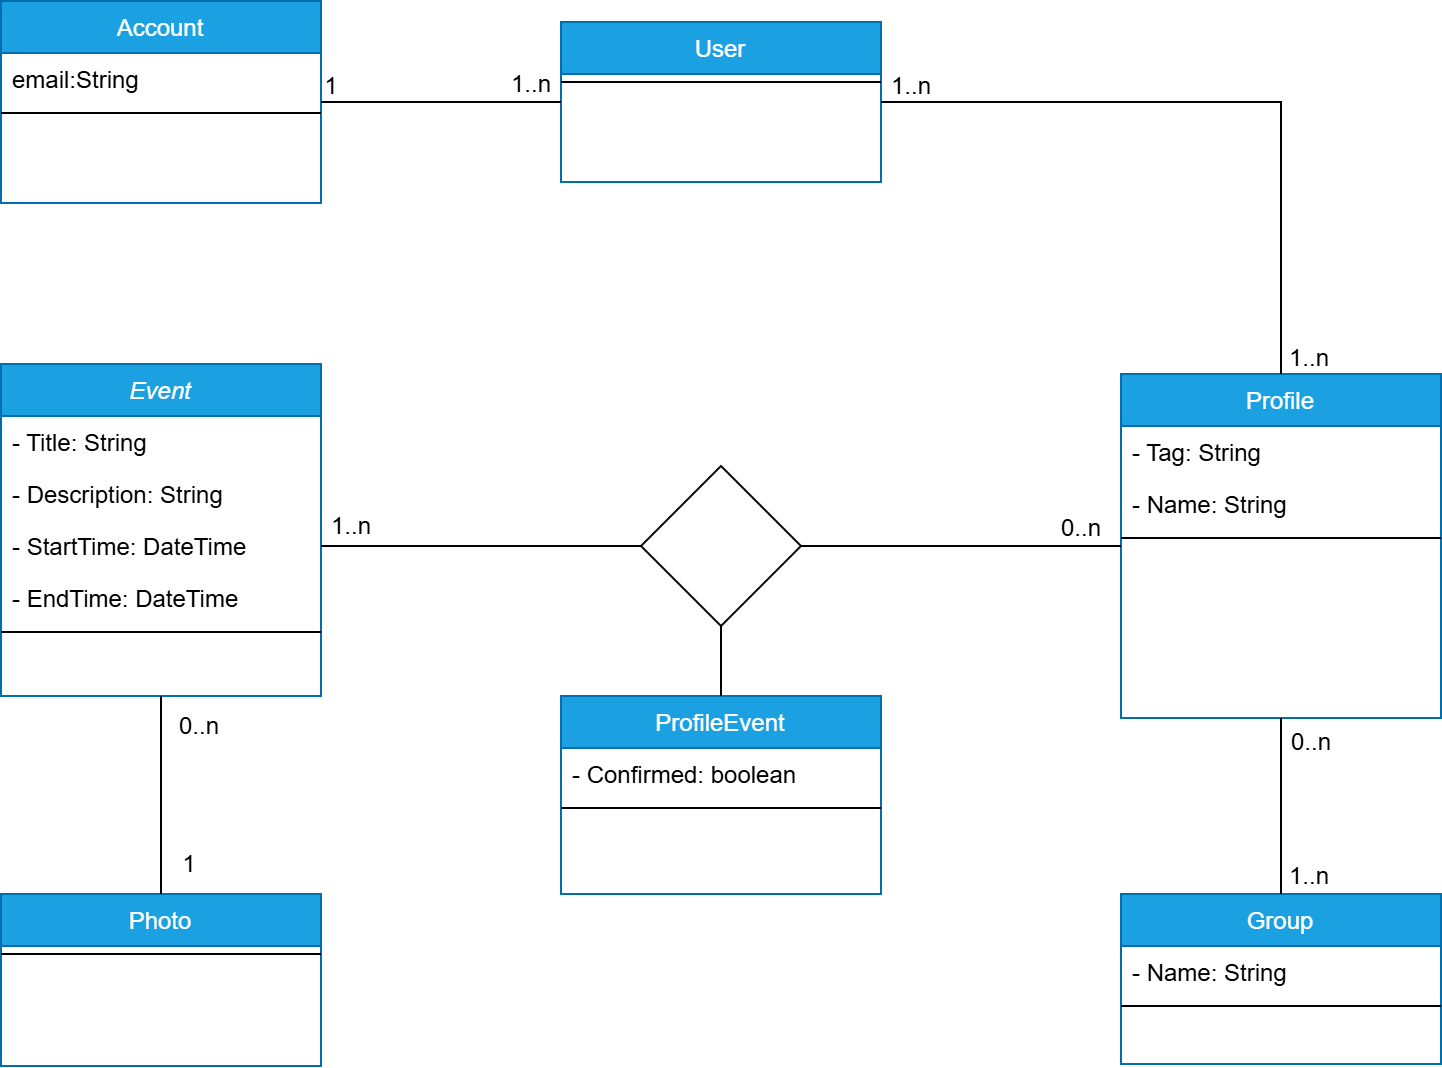
\includegraphics[width=\textwidth]{ModelloDominio.png}
    \end{center}
\end{figure}
\hfill \break

\newpage
\subsubsection{Architettura Logica: Struttura}
\hfill \break

\textbf{Diagramma dei package}
\hfill \break

\begin{figure}[h!]
    \begin{center}
        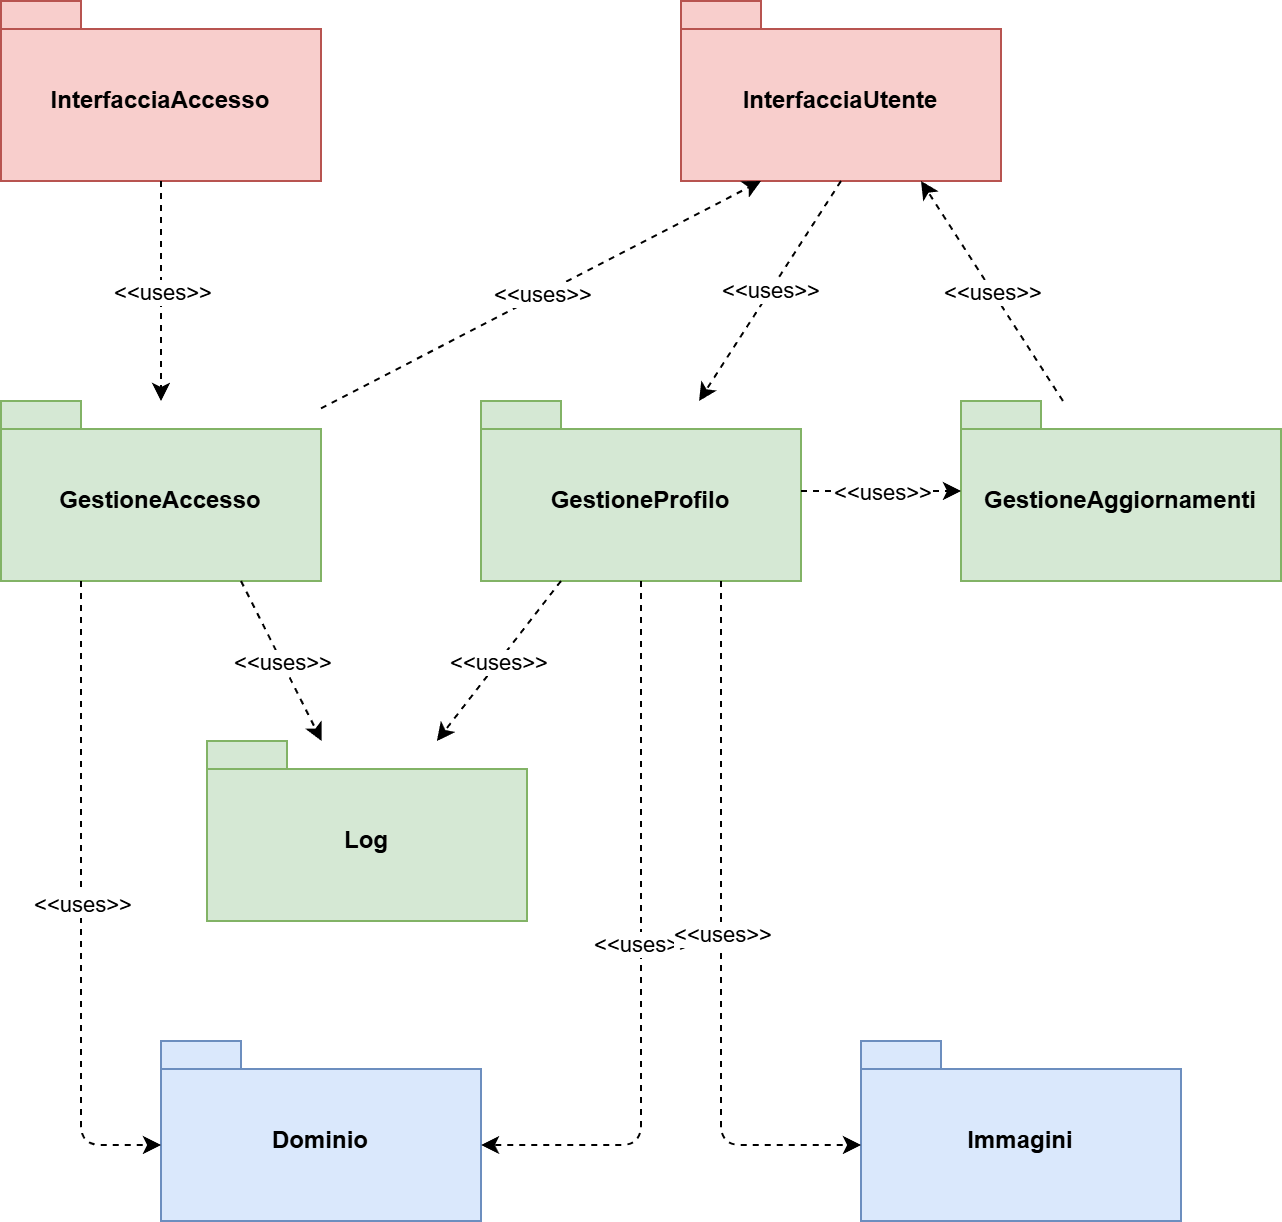
\includegraphics[width=\textwidth]{DiagrammaPackage.png}
    \end{center}
\end{figure}
\hfill \break

\textbf{Diagramma delle classi: Dominio}
\hfill \break

Non viene riportato il diagramma delle classi associato al package Dominio in quanto è il modello del dominio creato nella fase precedente.

\newpage

\textbf{Diagramma delle classi: InterfacciaAccesso \& GestioneAccesso}
\hfill \break

\begin{figure}[h!]
    \begin{center}
        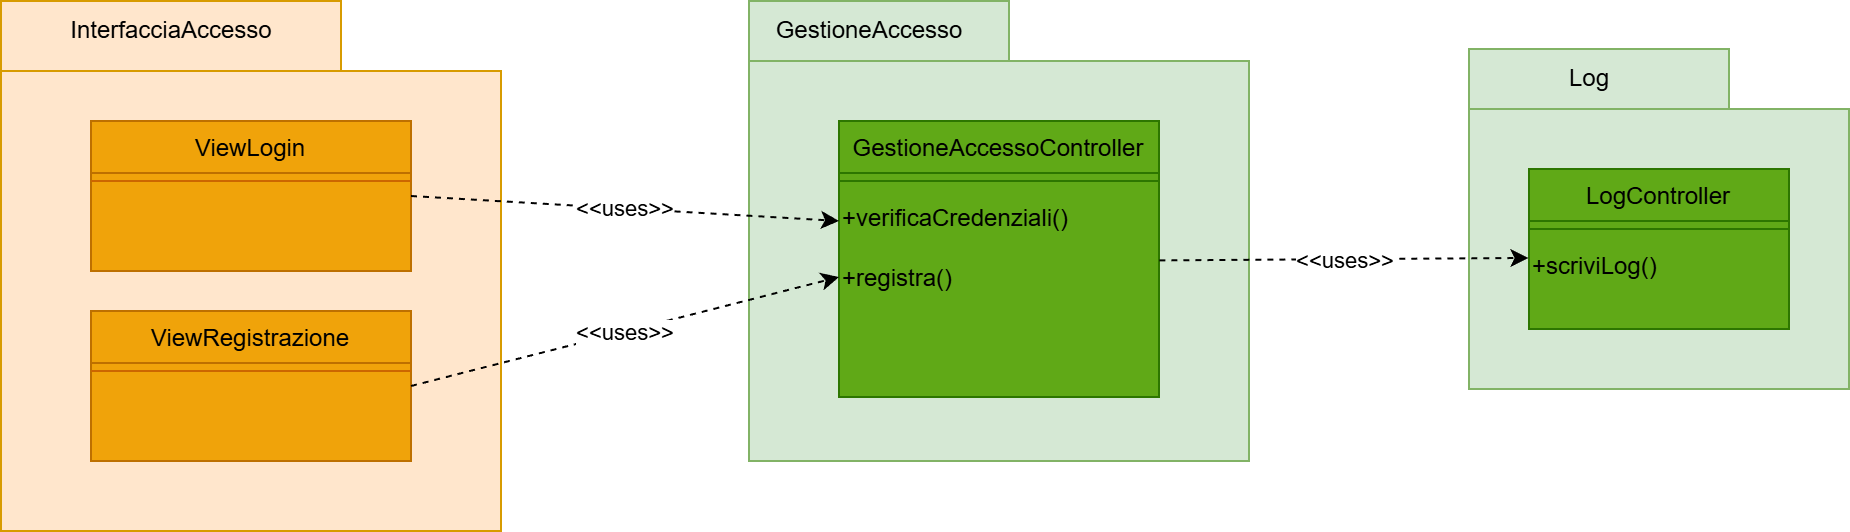
\includegraphics[width=\textwidth]{GestioneAccesso.png}
    \end{center}
\end{figure}
\hfill \break

\textbf{Diagramma delle classi: InterfacciaUtente \& GestioneProfilo \& GestioneAggiornamenti }

\begin{figure}[h!]
    \begin{center}
        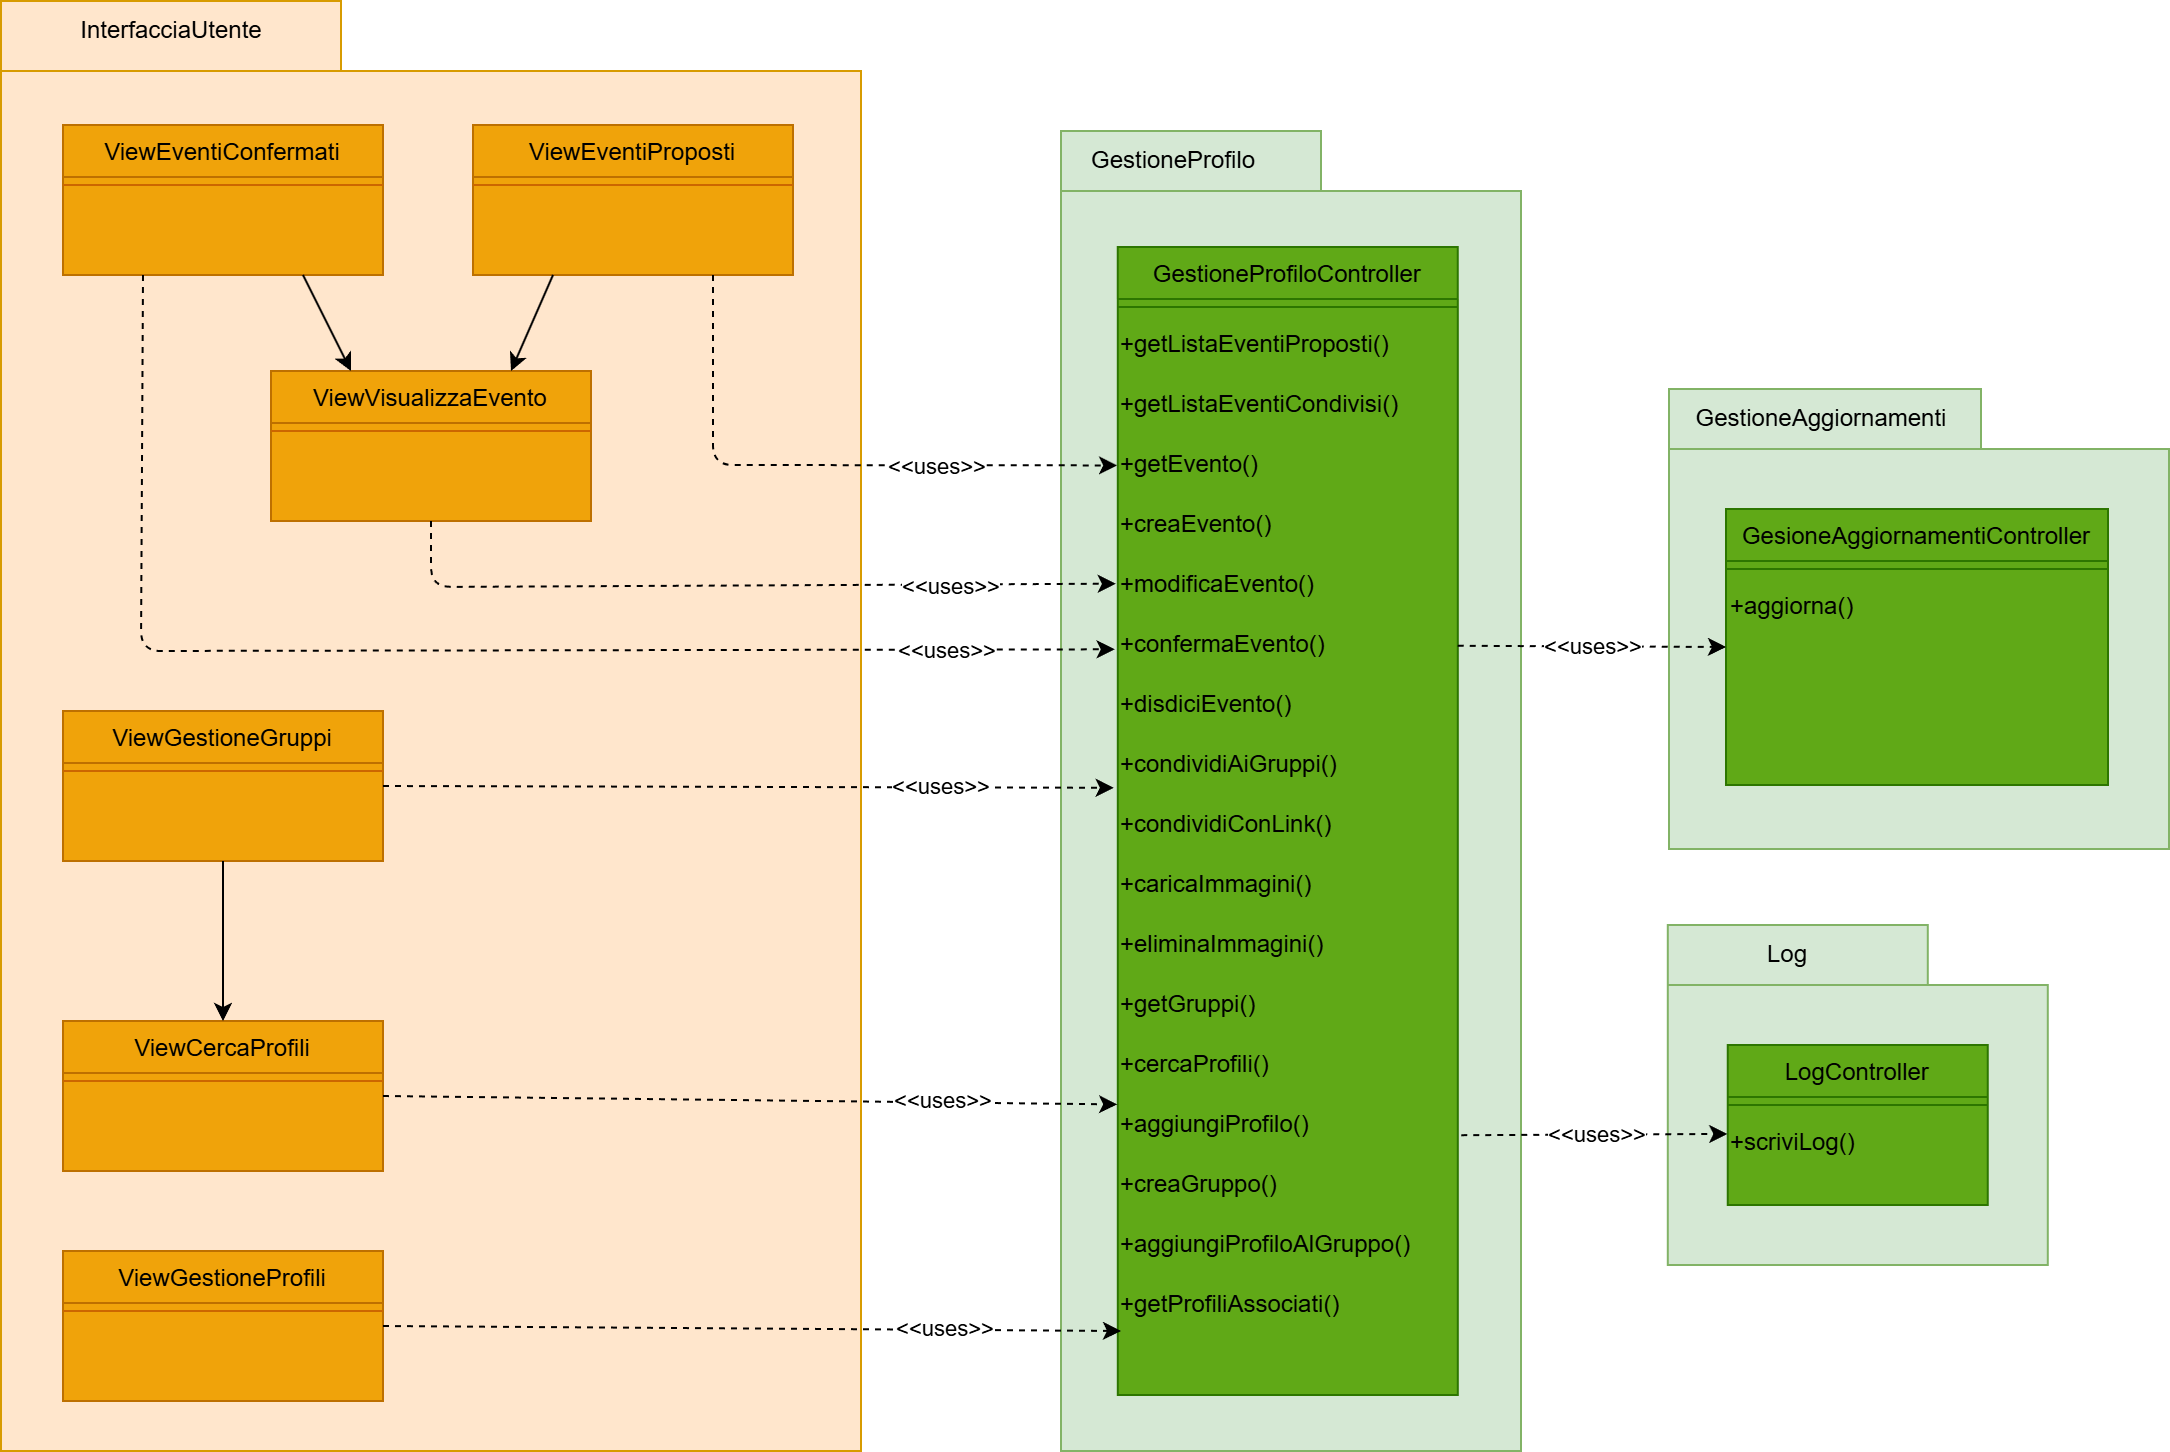
\includegraphics[width=\textwidth]{GestioneProfilo.png}
    \end{center}
\end{figure}
\hfill \break
\newpage

\subsubsection{Architettura Logica: Interazione}

In seguito saranno riportati i principali diagrammi di sequenza durante un normale utilizzo dell'applicazione.
\hfill \break

\textbf{Diagramma di Sequenza: Login Utente}

\begin{figure}[h!]
    \begin{center}
        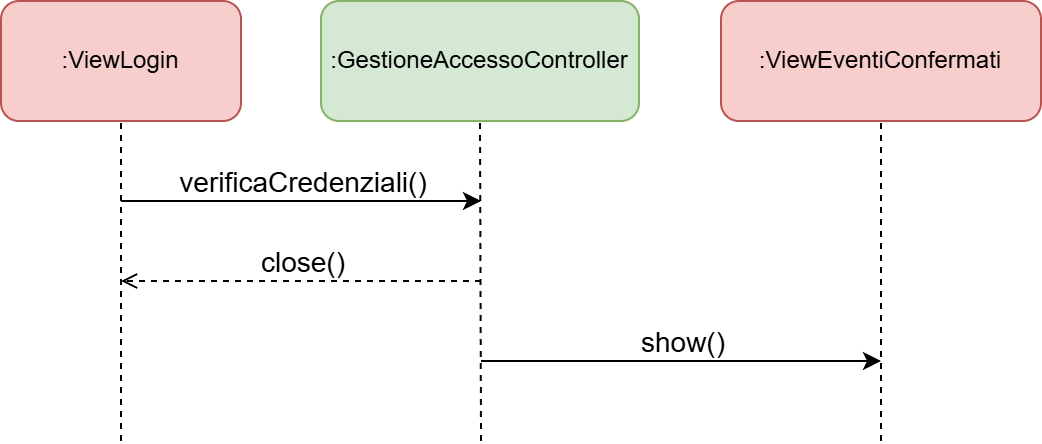
\includegraphics[width=\textwidth]{SequenzaLogin.png}
    \end{center}
\end{figure}
\hfill \break

\textbf{Diagramma di Sequenza: Registrazione}

\begin{figure}[h!]
    \begin{center}
        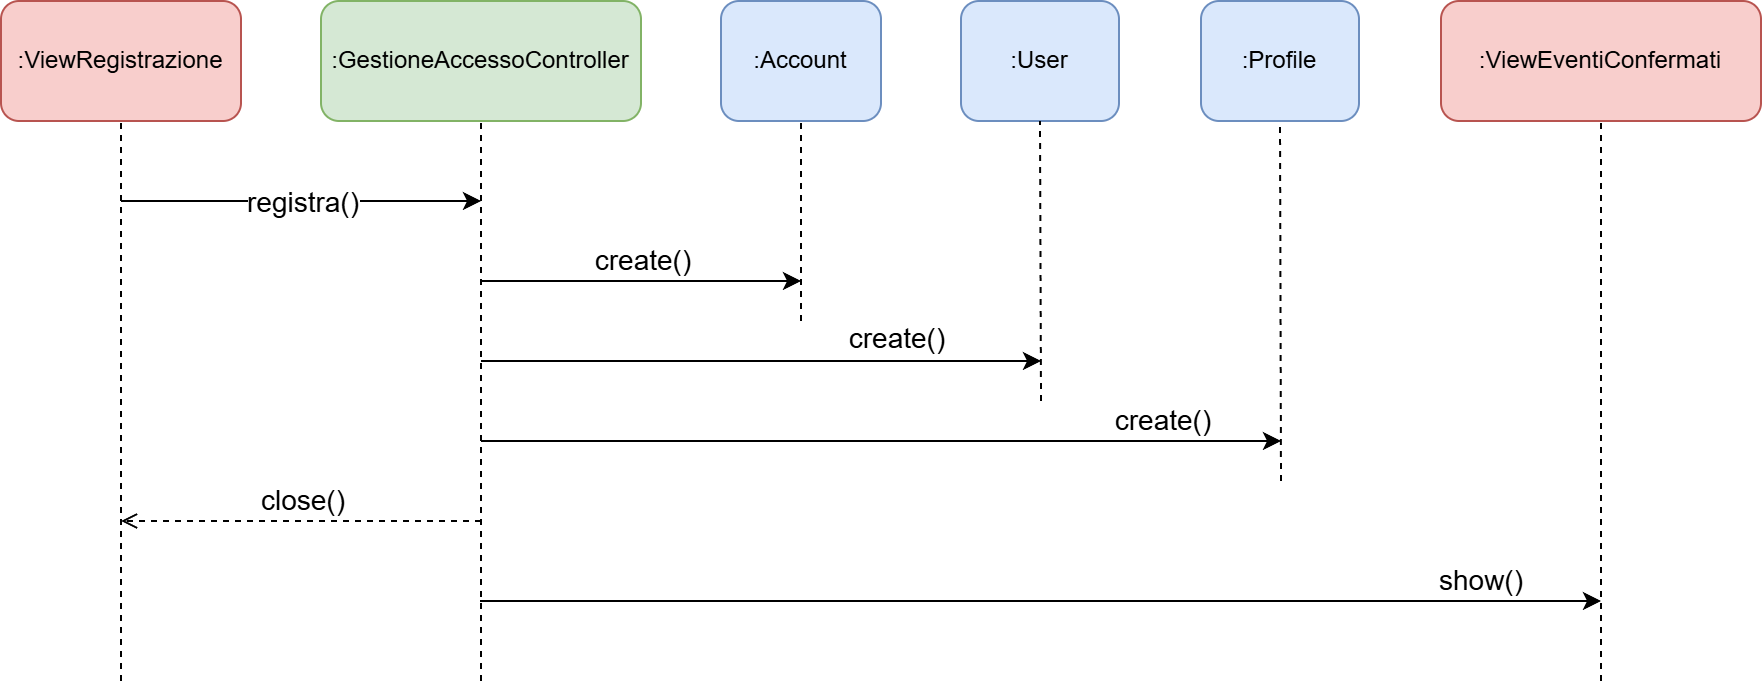
\includegraphics[width=\textwidth]{SequenzaRegistrazione.png}
    \end{center}
\end{figure}
\hfill \break
\newpage

\textbf{Diagramma di Sequenza: Visualizza Eventi Confermati}

\begin{figure}[h!]
    \begin{center}
        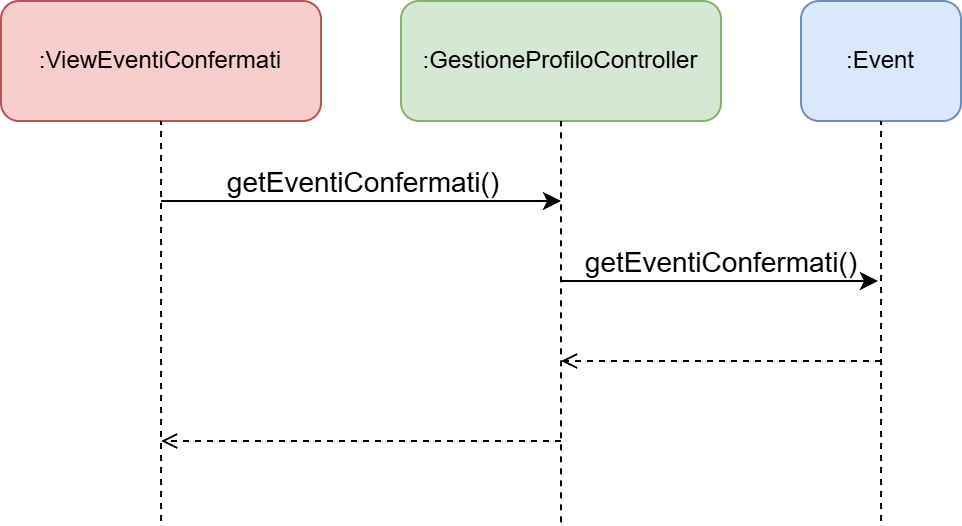
\includegraphics[width=\textwidth]{SequenzaVisualizzaEventiConfermati.png}
    \end{center}
\end{figure}
\hfill \break

\textbf{Diagramma di Sequenza: Visualizza Eventi Proposti}

\begin{figure}[h!]
    \begin{center}
        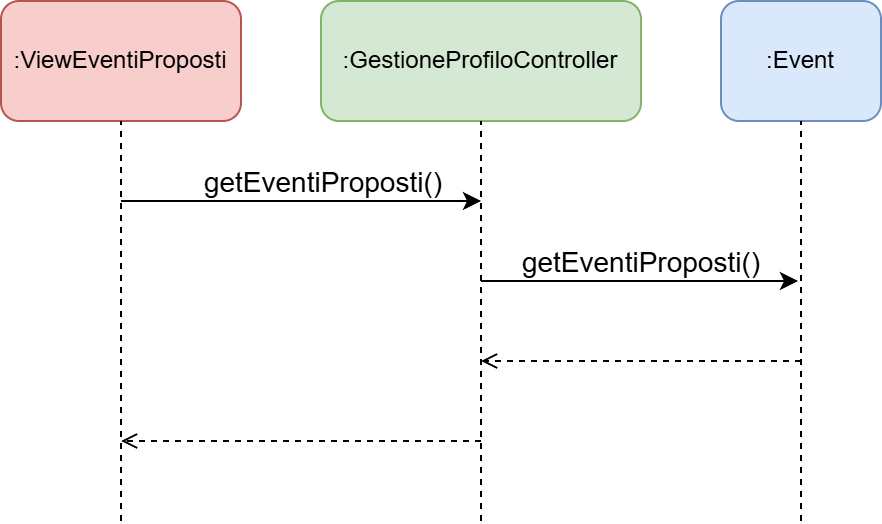
\includegraphics[width=\textwidth]{SequenzaVisualizzaEventiProposti.png}
    \end{center}
\end{figure}
\hfill \break
\newpage
\textbf{Diagramma di Sequenza: Visualizza Evento}

\begin{figure}[h!]
    \begin{center}
        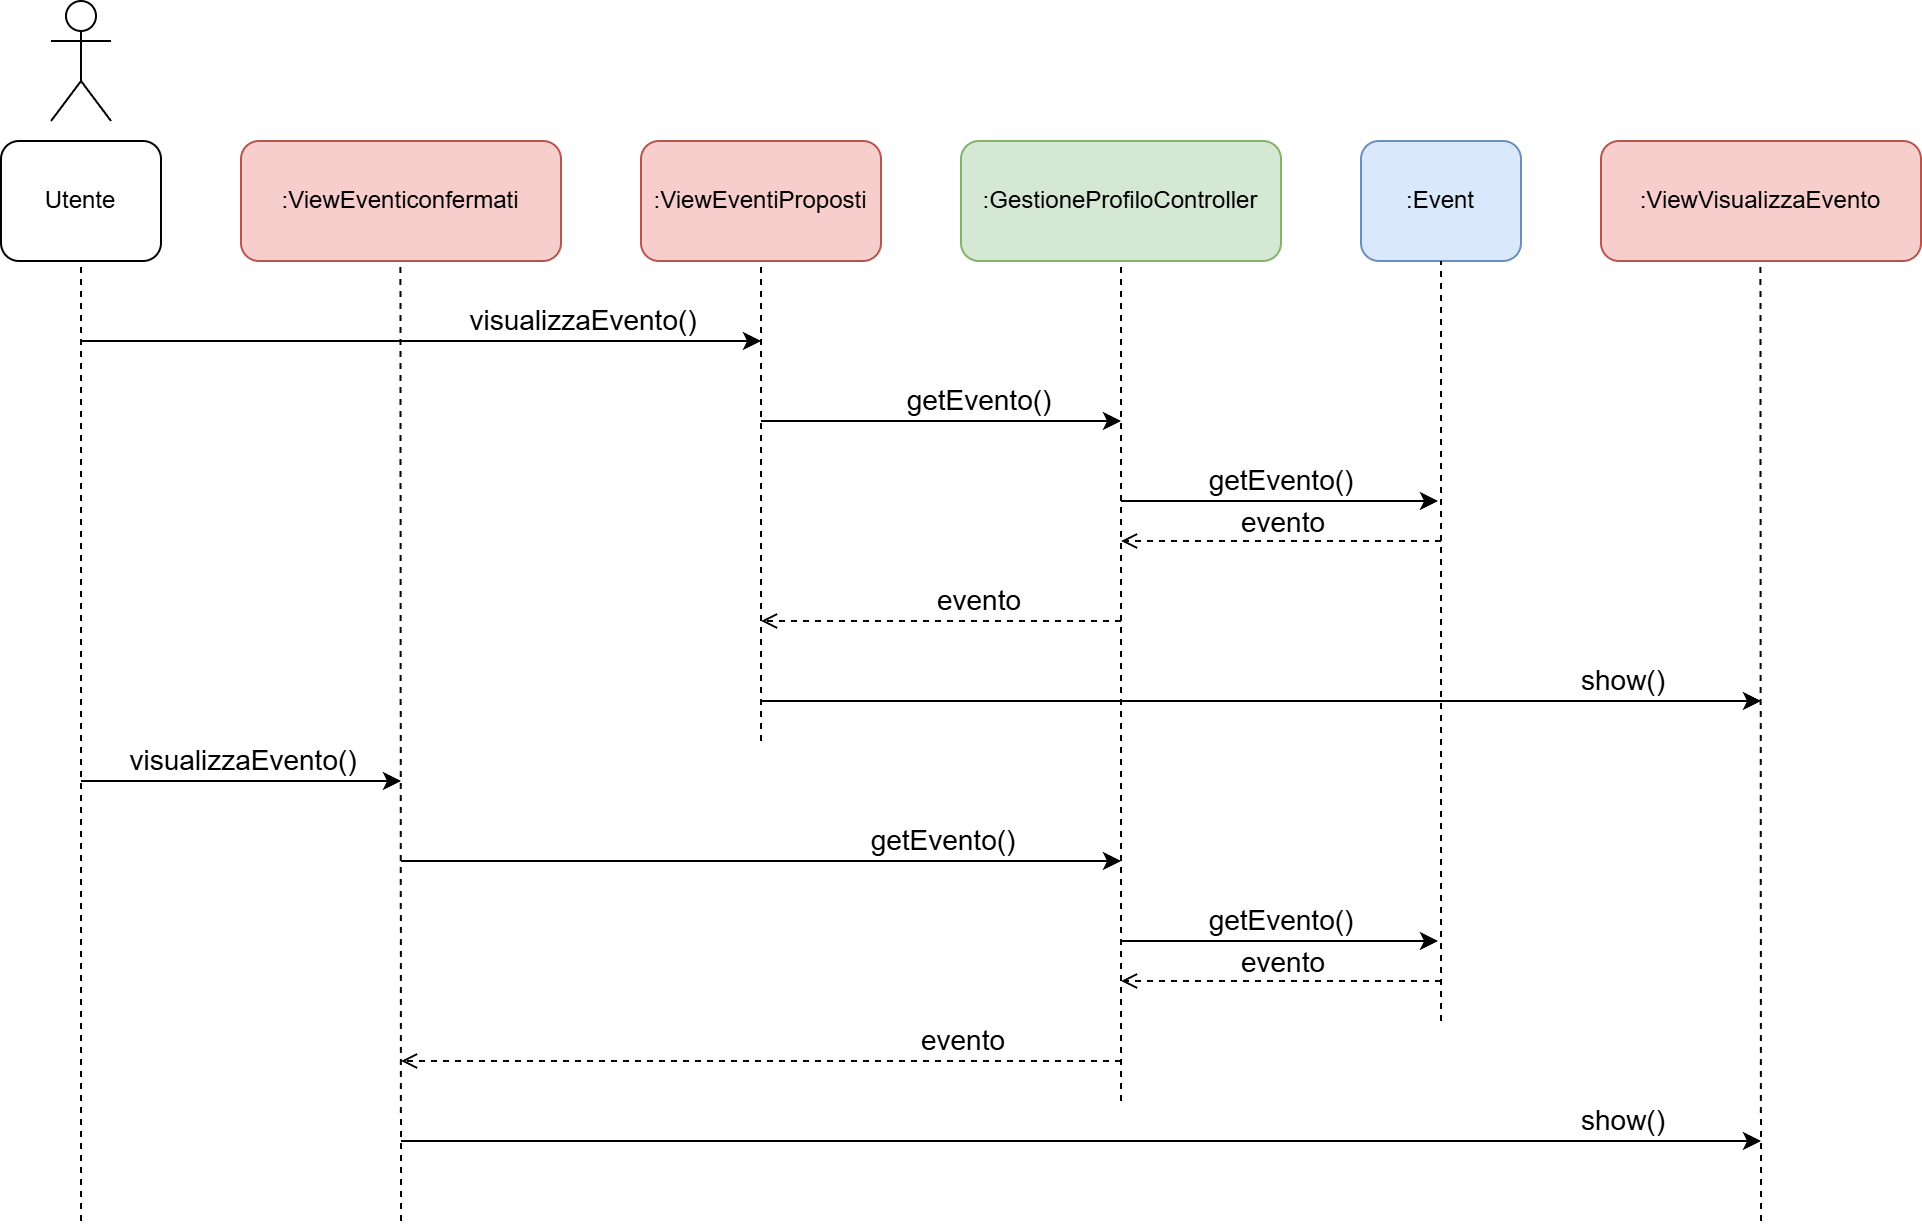
\includegraphics[width=\textwidth]{SequenzaVisualizzaEvento.png}
    \end{center}
\end{figure}
\hfill \break
\textbf{Diagramma di Sequenza: Condividi Evento ai gruppi}

\begin{figure}[h!]
    \begin{center}
        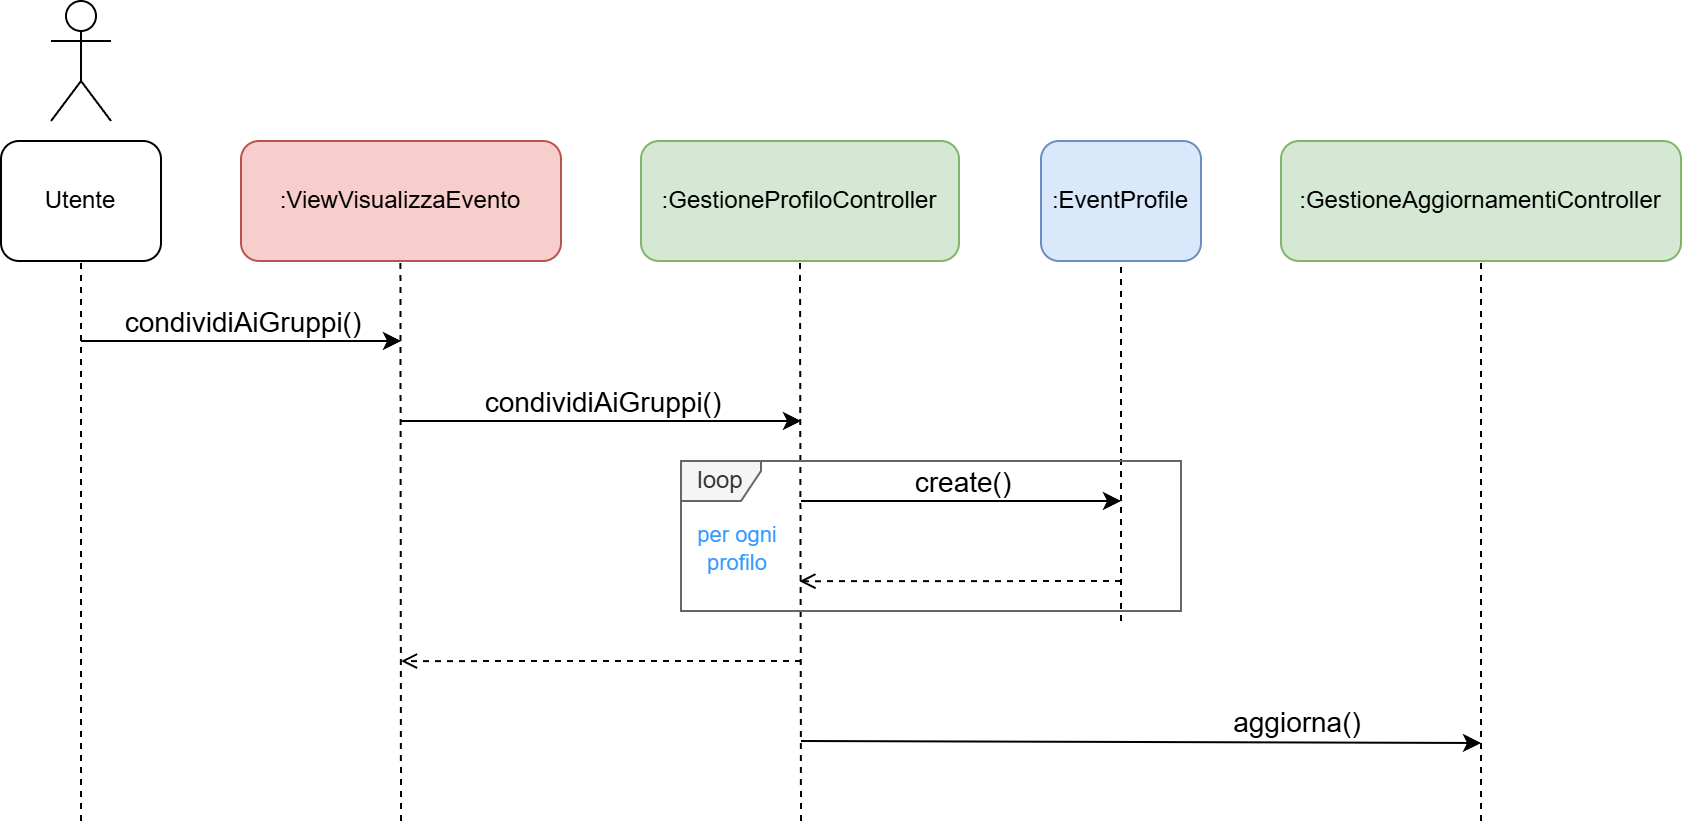
\includegraphics[width=\textwidth]{SequenzaCondividiEvento.png}
    \end{center}
\end{figure}
\hfill \break
\clearpage

\textbf{Diagramma di Sequenza: Crea / Modifica / Conferma / Disdici Evento}

\begin{figure}[h!]
    \begin{center}
        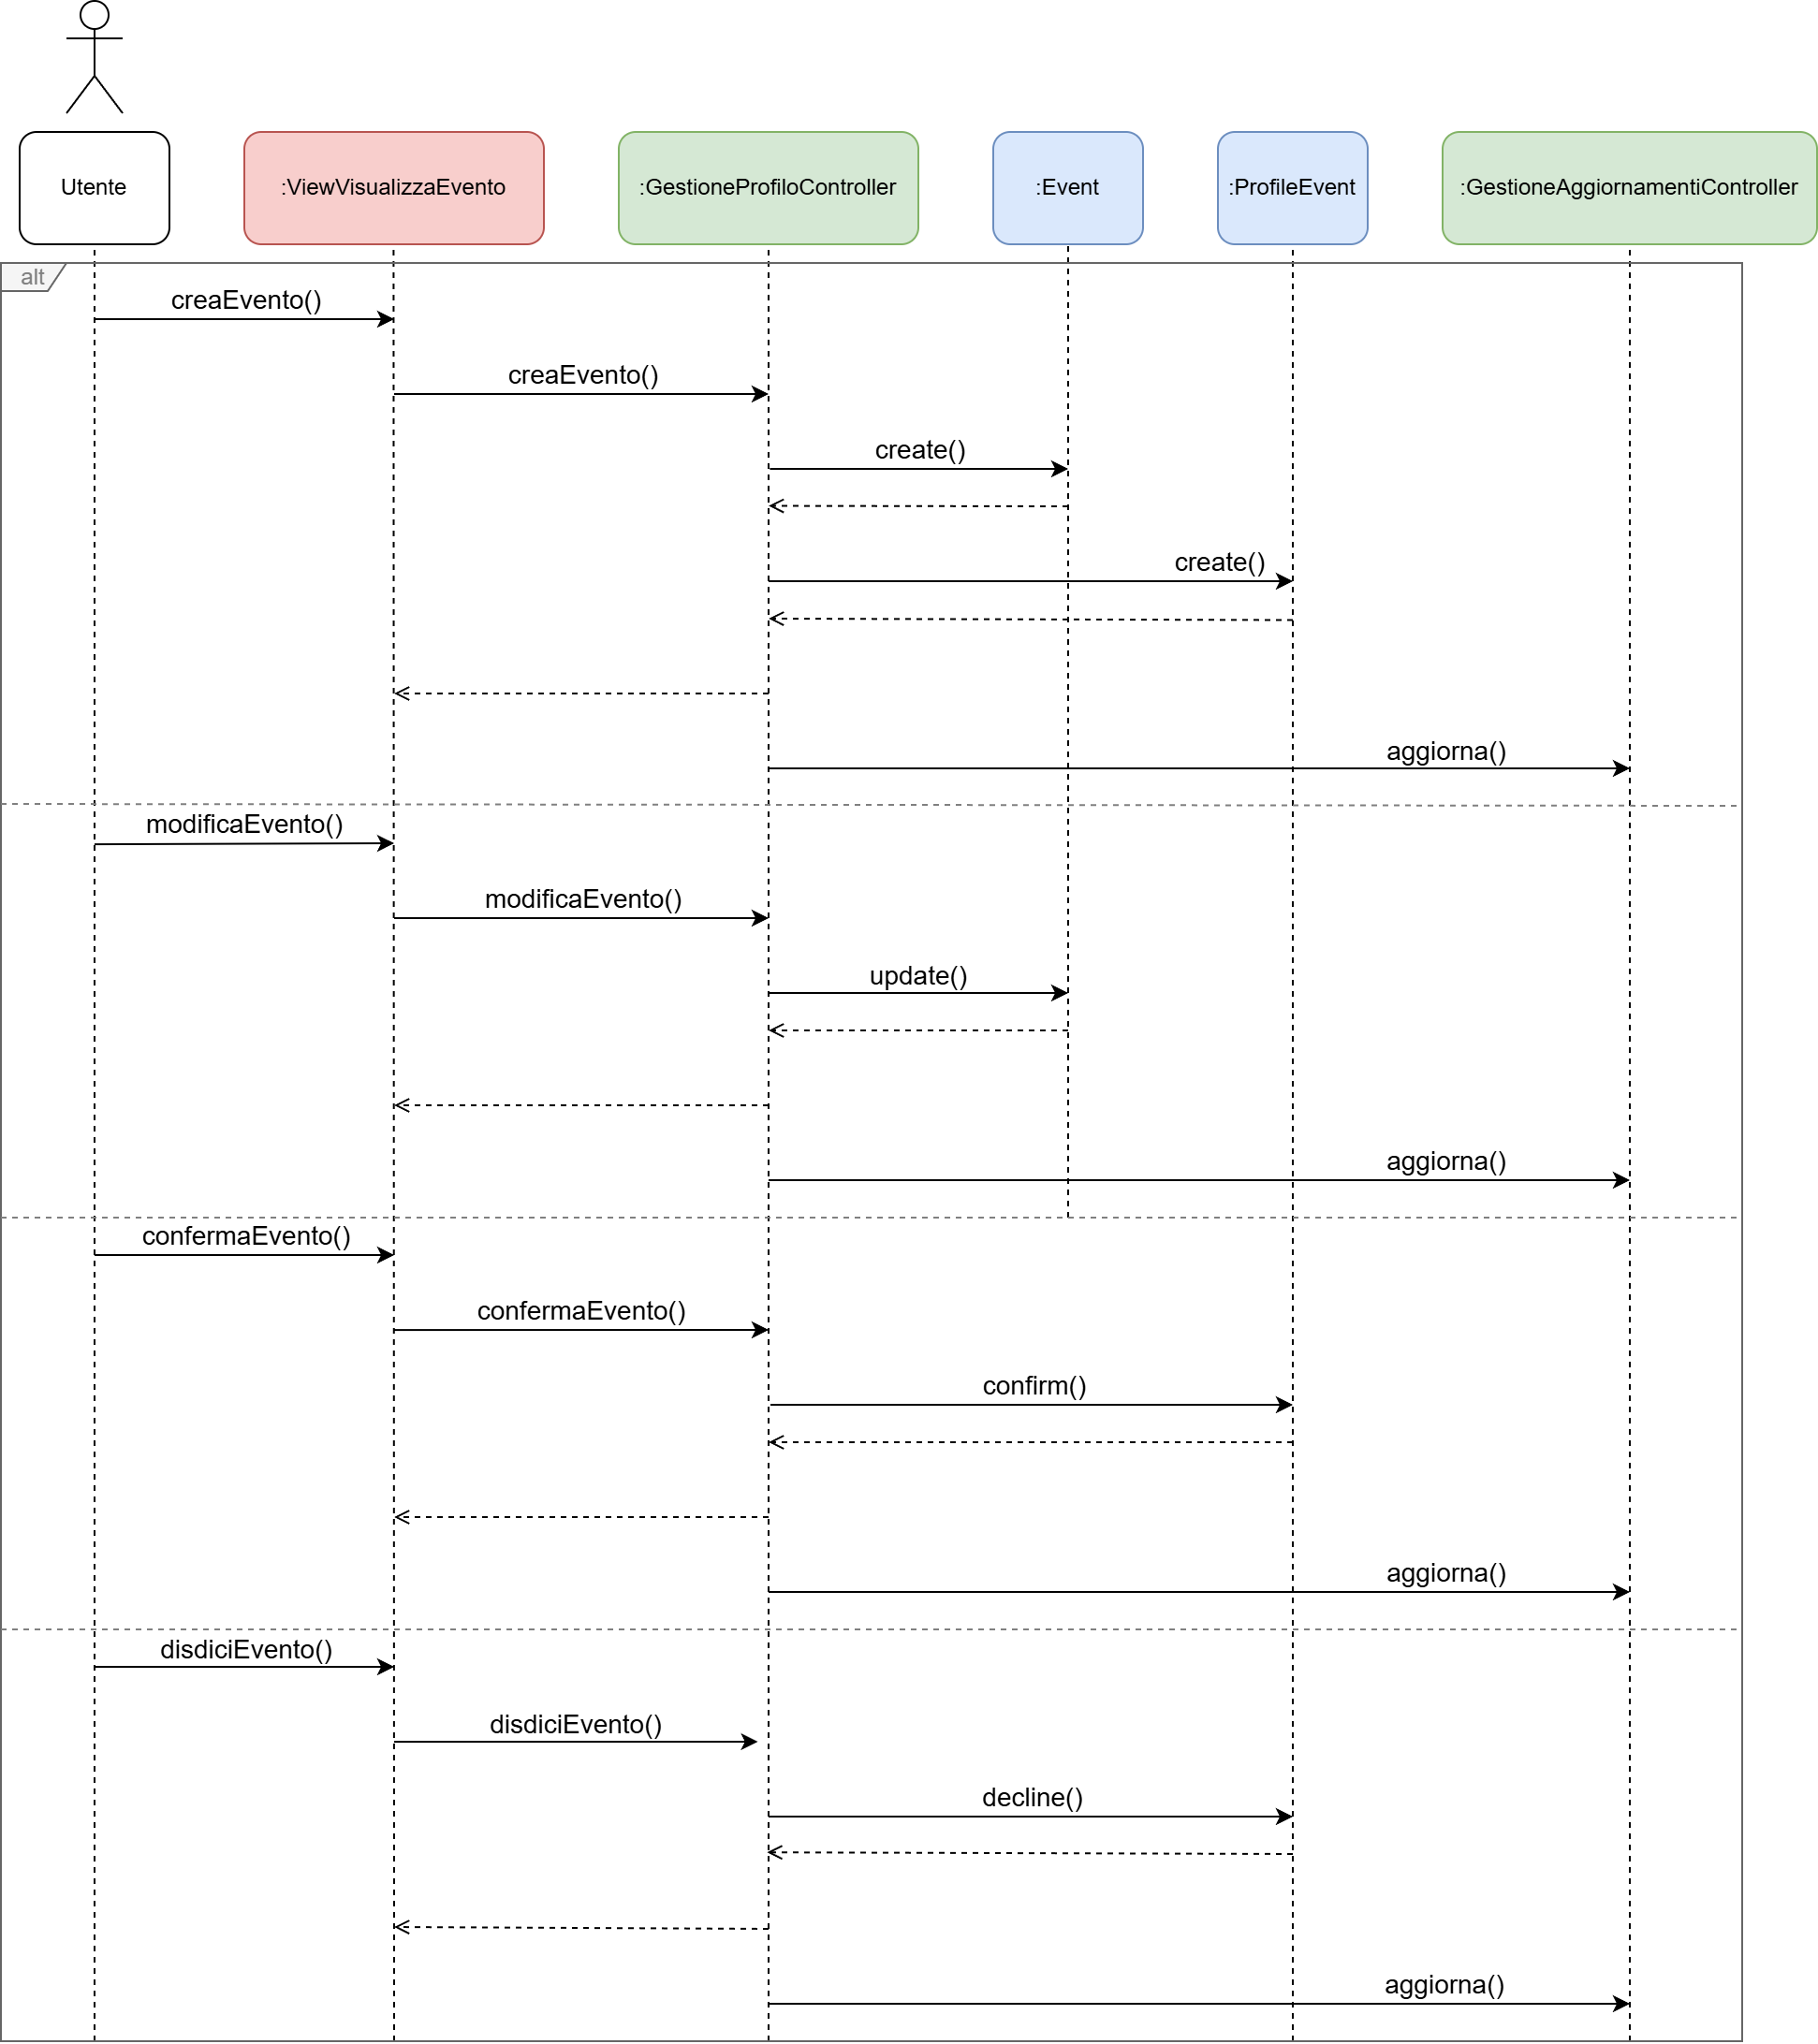
\includegraphics[width=\textwidth]{SequenzaCreaModificaEvento.png}
    \end{center}
\end{figure}
\hfill \break
\clearpage
\textbf{Diagramma di Sequenza: Carica Immagini}

\begin{figure}[h!]
    \begin{center}
        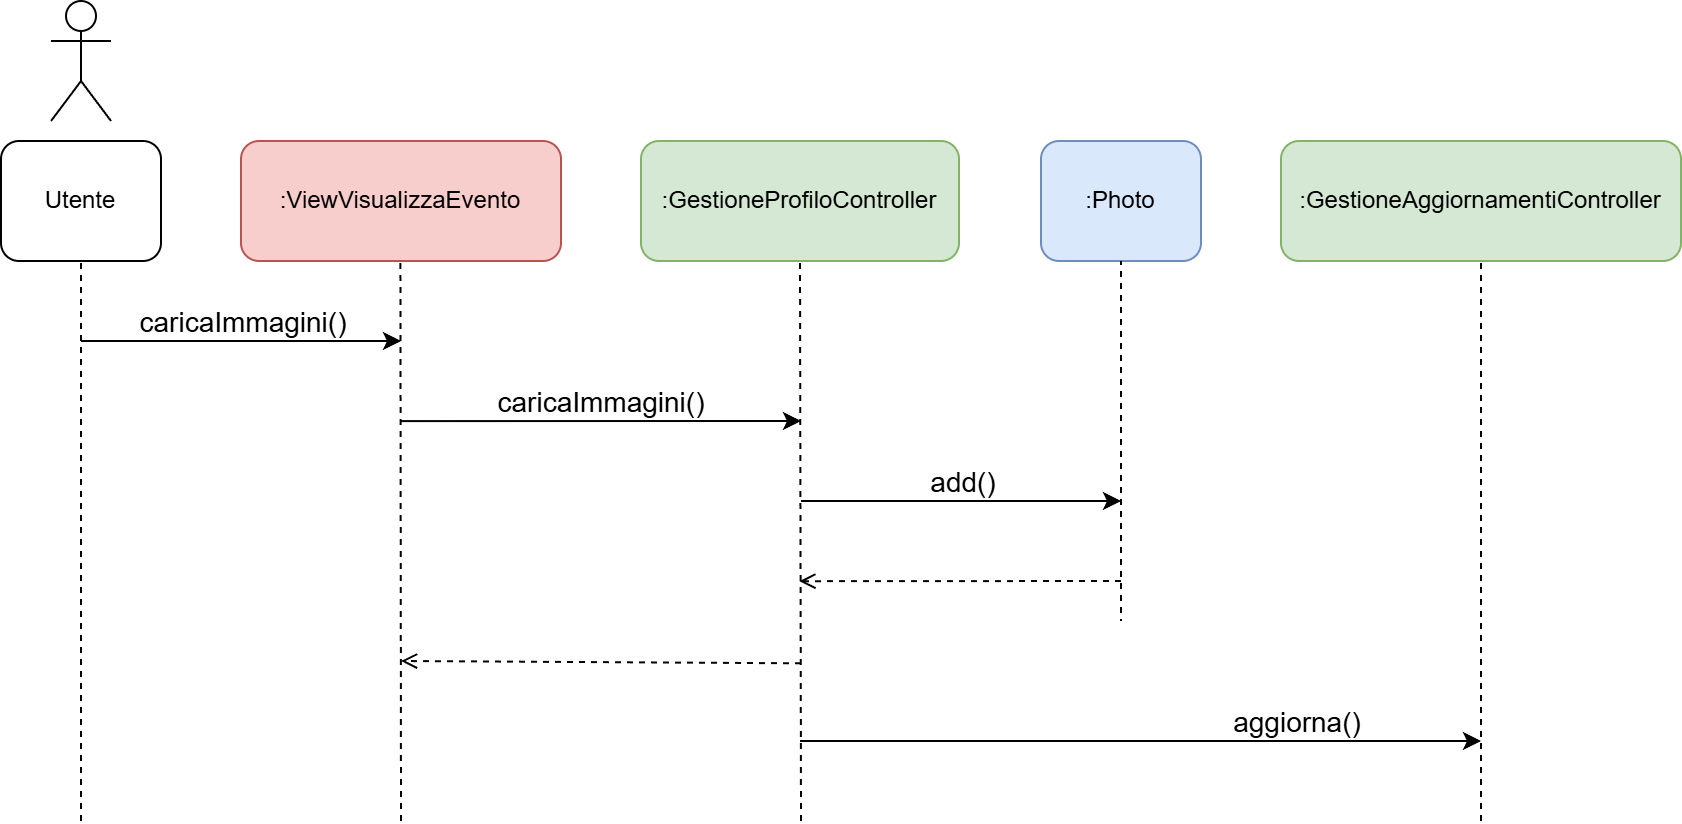
\includegraphics[width=\textwidth]{SequenzaCaricaImmagini.png}
    \end{center}
\end{figure}
\hfill \break

\textbf{Diagramma di Sequenza: Recupera Immagini}

\begin{figure}[h!]
    \begin{center}
        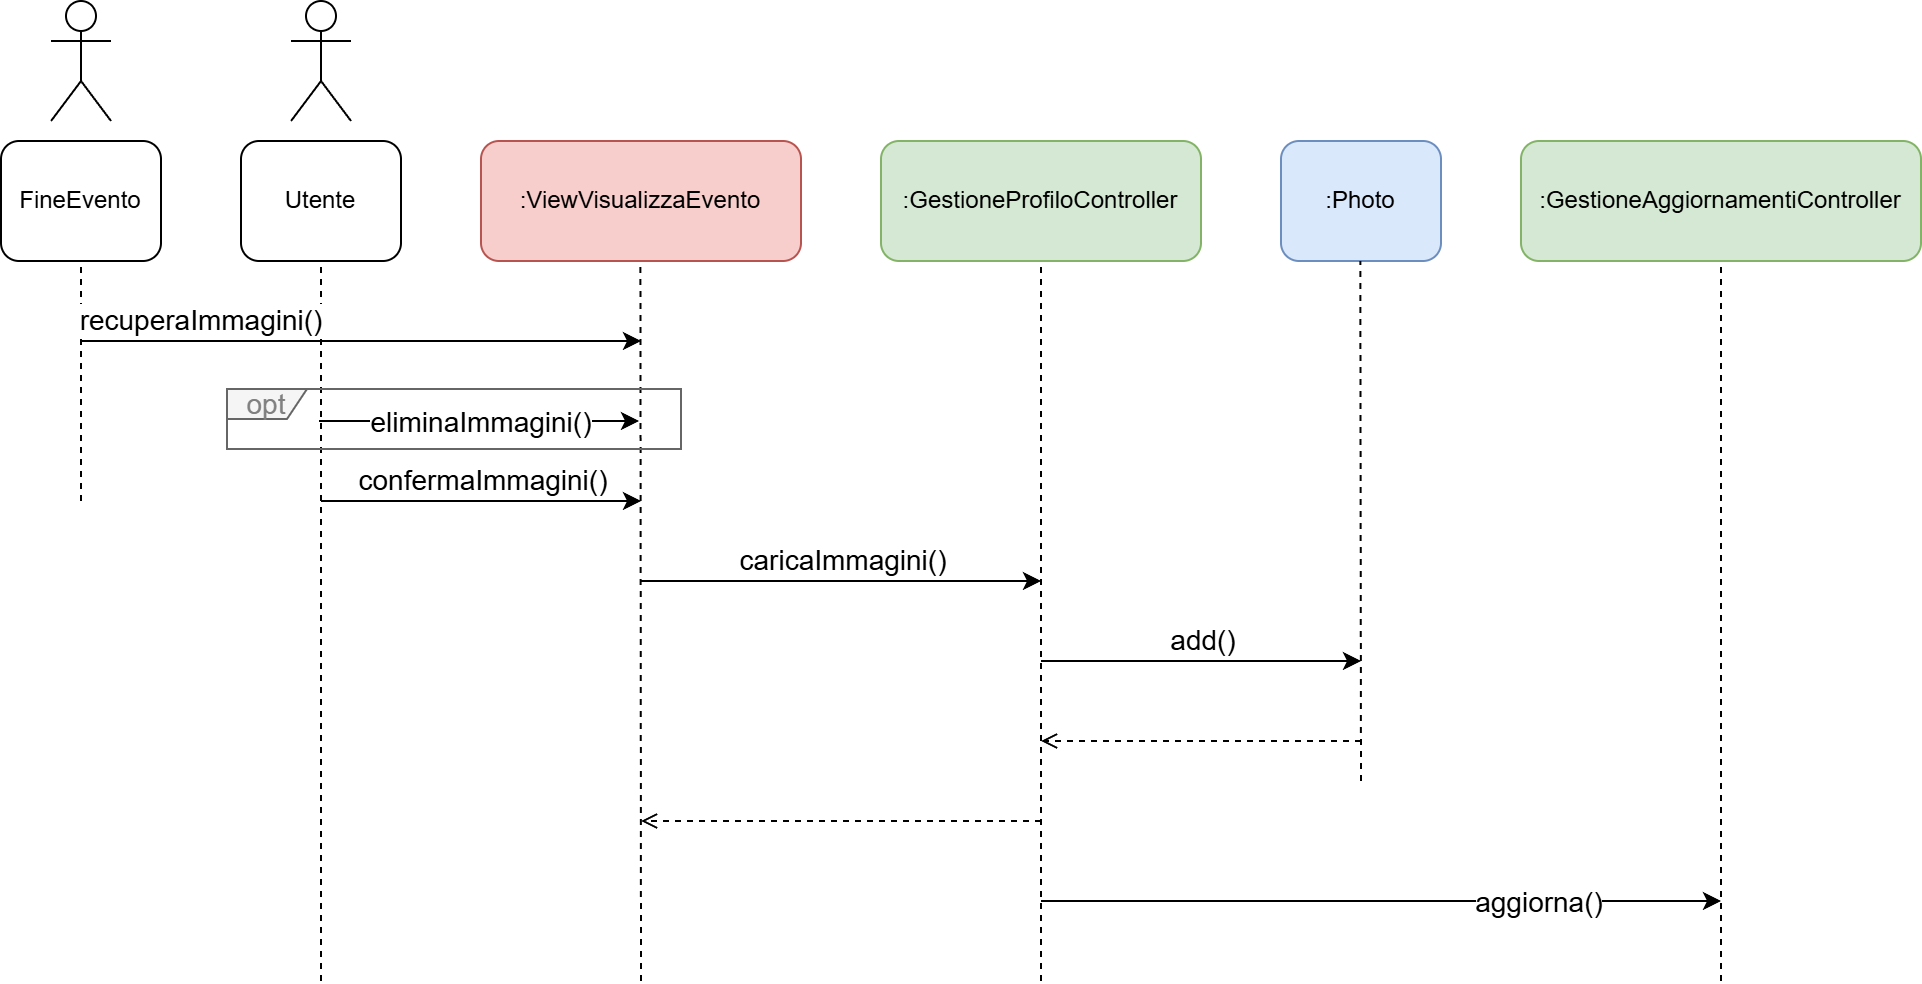
\includegraphics[width=\textwidth]{SequenzaConfermaImmagini.png}
    \end{center}
\end{figure}
\hfill \break
\clearpage

\newpage

\subsubsection{Piano di Lavoro}

I compiti sono stati divisi in base alle competenze di
ogni membro del gruppo come indicato nella tabella sottostante:
\hfill \break

\begin{tabular} {|P{6cm}|P{4.5cm}|P{4.5cm}|}
    \hline
    \textbf{Package}      & \textbf{Progetto} & \textbf{Sviluppo} \\
    \hline
    GestioneAccesso       & Romanini          & Romanini          \\
    \hline
    GestioneEventi        & Romanini          & Romanini          \\
    \hline
    GestioneAggiornamenti & Romanini          & Romanini          \\
    \hline
    InterfacciaUtente     & Romanini          & Romanini          \\
    \hline
    InterfacciaAccesso    & Romanini          & Romanini          \\
    \hline
    Dominio               & Romanini          & Romanini          \\
    \hline
    Immagini              & Romanini          & Romanini          \\
    \hline
    Log                   & Romanini          & Romanini          \\
    \hline
\end{tabular}
\hfill \break

I tempi di rilascio sono i seguenti:
\begin{itemize}
    \item Progettazione entro due settimane dalla data odierna
    \item Sviluppo dei vai moduli con annessi test unitari entro due mesi dalla fine della fase di progettazione
    \item Integrazione e testing del sistema entro un mese dalla fine dello sviluppo
\end{itemize}
\hfill \break

\subsubsection{Sviluppi Futuri}
Gli sviluppi futuri potranno comprendere, in base a decisioni di marketing:
\begin{itemize}
    \item La visualizzazione degli impegni degli altri profili
    \item L'implementazione di una chat per ogni gruppo
    \item Sviluppo di strumenti utili all'organizzazione dei gruppi, quali:
          \begin{itemize}
              \item form per combinare le disponibilità reciproche
              \item appunti condivisi(liste della spesa o note su chi porta cosa)
              \item calcolo delle spese compiute da ciascun componente
          \end{itemize}
    \item La creazione di profili pubblici che possono essere seguiti
    \item La creazione di eventi pubblici
    \item Una funzionalità di ricerca degli eventi pubblici
    \item Supporto alla gestione di prenotazione e organizzazione degli eventi, dalle liste di attesa alla vendita dei biglietti
    \item La possibilità per le aziende di gestire in locale il proprio server e i relativi dati
\end{itemize}

